\subsection{Granularity of Variability}
% Christian's paper?
% empirical studies?
% essence: file-level variability is not engough

\subsection{What is a Preprocessor?}
% compiler, compile-time
% when to run a preprocessor
% the preprocessing principle: hide code from the compiler
% language independent

% in-place vs outa-place preprocessors
% how to select features? parameters passed to the preprocessor, define in source code

\subsection{CPP -- The C Preprocessor}
\begin{frame}{\myframetitle\ -- In a Nutshell \mytitlesource{\featureide}}
	\leftorright{
		\myexampletight{Example Input to the Preprocessor}{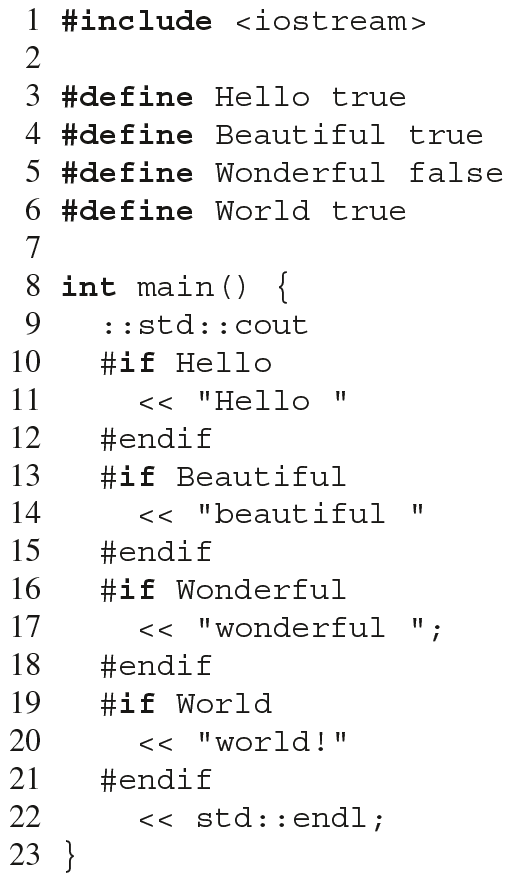
\includegraphics[scale=.3]{preprocessor-c}}
	}{
		\myexampletight{Example Output (Simplified)}{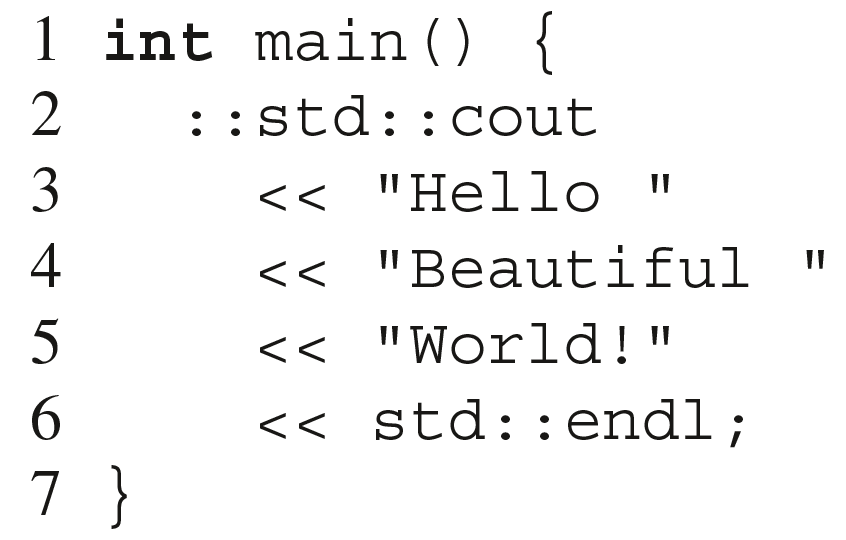
\includegraphics[scale=.15]{preprocessor-c-output}}
	}
\end{frame}
% TODO #if in above example? does this work?
% TODO keywords: #ifdef #endif #else
% TODO illustrate parameters and the call of the preprocessor

\begin{frame}{\myframetitle\ -- In a Coconutshell}
	\todots
\end{frame}
% TODO explain the most important commands: #if #defined or and not ... #elif
% TODO #include

% TODO #error
% TODO parameters, #define, even combinations

% TODO single characters
% TODO discipliced, undisciplined

\subsection{Preprocessors for Java}
\begin{frame}{Munge -- A Simple Preprocessor for Java \mytitlesource{\featureide}}
	\leftorright{
		\myexampletight{Example Input and Output}{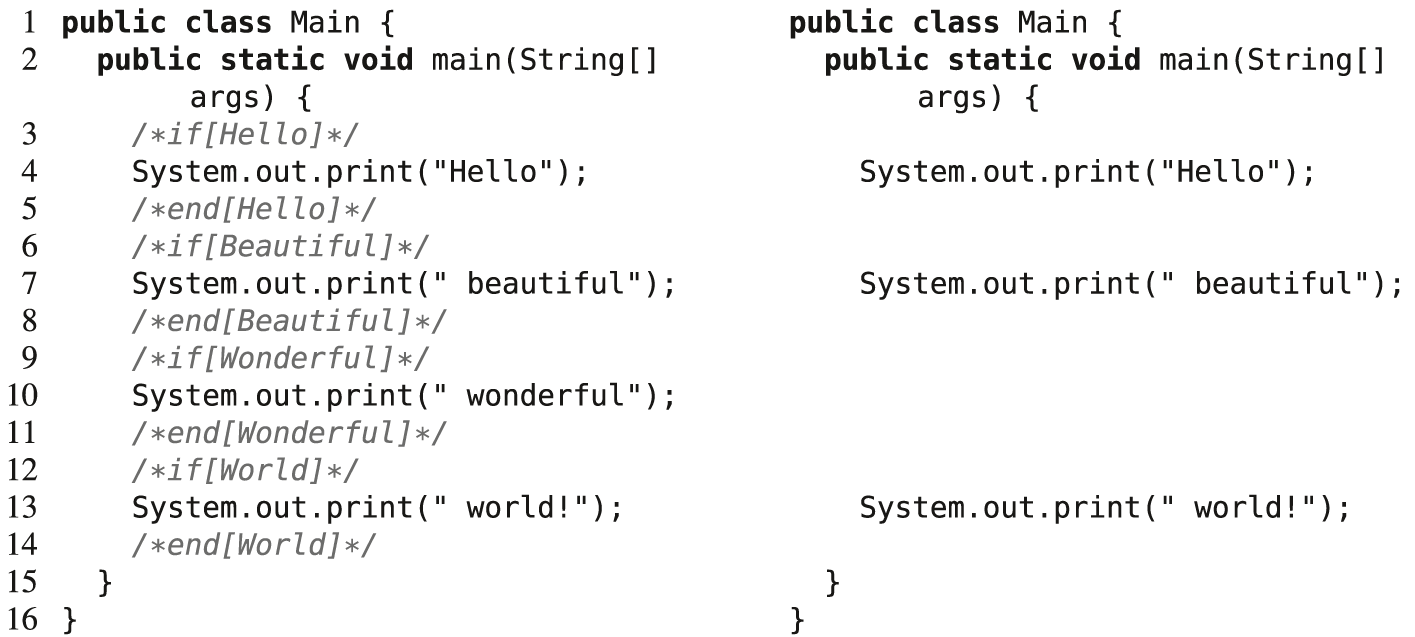
\includegraphics[width=\linewidth]{preprocessor-munge}}
	}{
		\myexampletight{Calling the Preprocessor}{
			\centering
			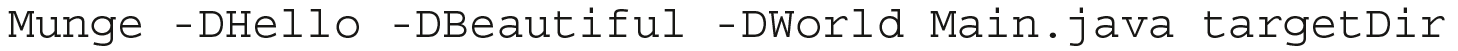
\includegraphics[width=\linewidth]{preprocessor-munge-call}
			
			~
			
			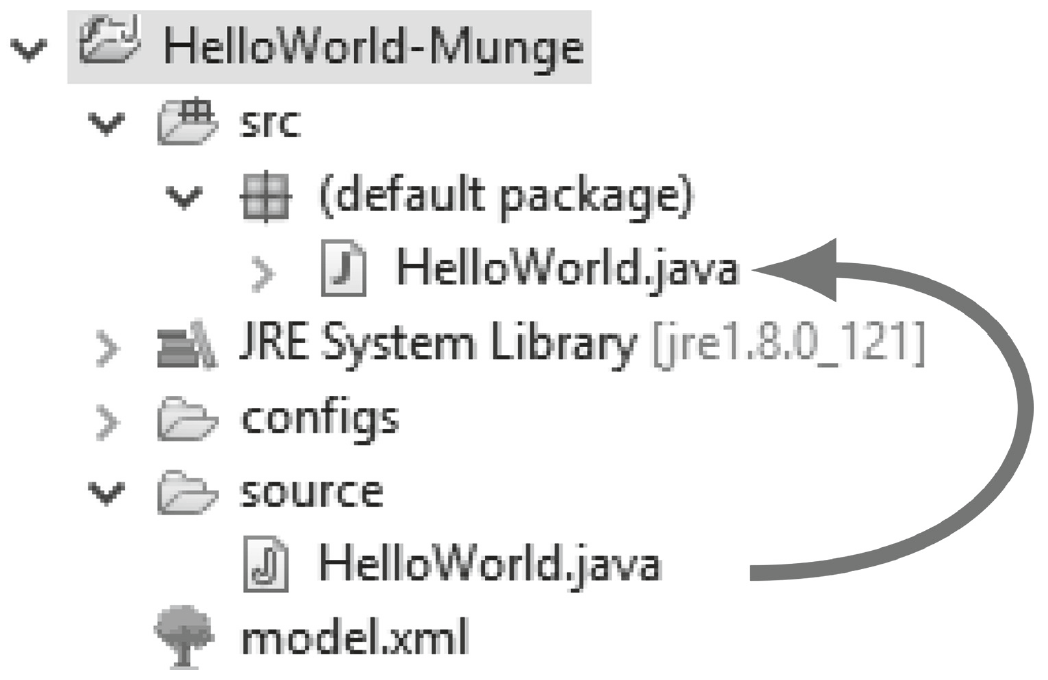
\includegraphics[width=.7\linewidth]{preprocessor-munge-idea}
		}
	}
\end{frame}

\begin{frame}{Antenna -- An In-Place Preprocessor for Java \mytitlesource{\featureide}}
	\leftorright{
		\myexampletight{Example Input and Output}{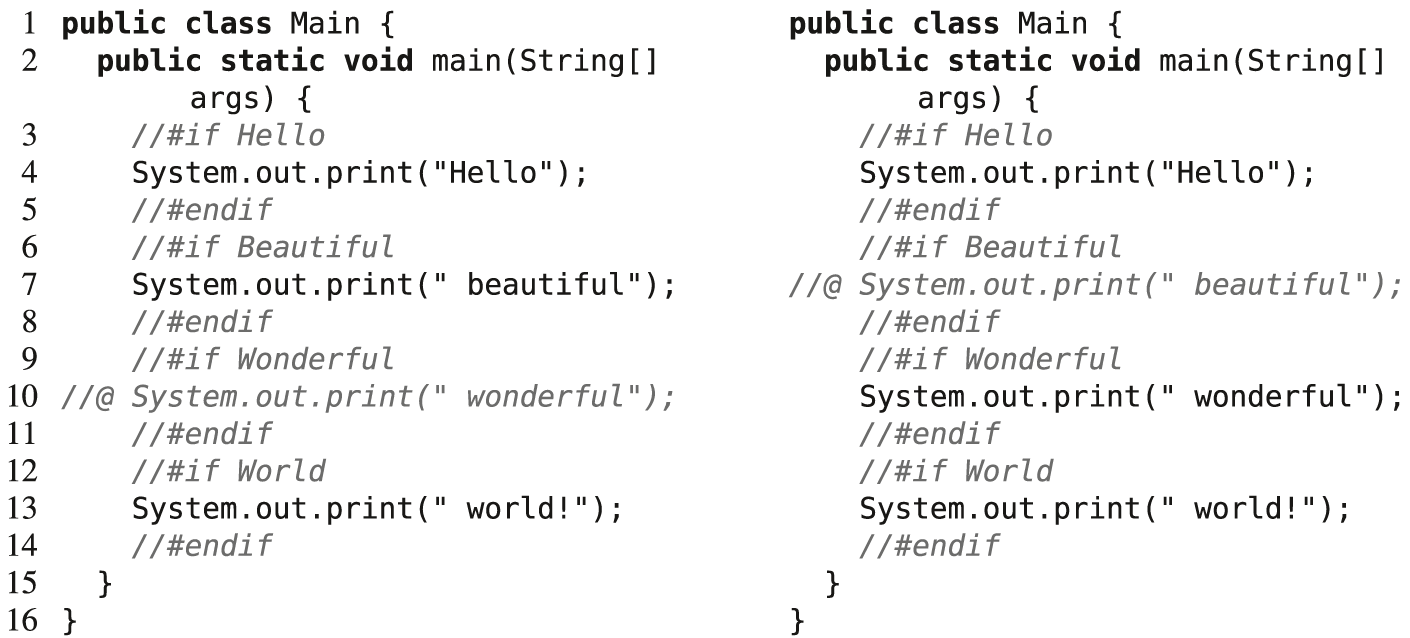
\includegraphics[width=\linewidth]{preprocessor-antenna}}
	}{
		\myexampletight{Calling the Preprocessor}{
			\centering
			
\includegraphics[width=\linewidth]{preprocessor-antenna-call}
			
			~
			
			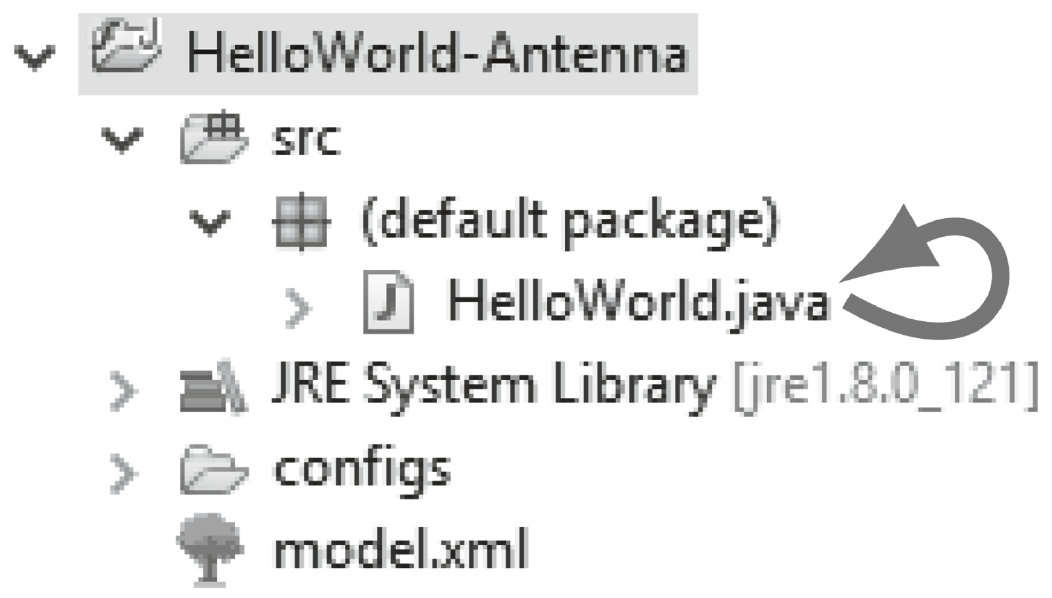
\includegraphics[width=.7\linewidth]{preprocessor-antenna-idea}
		}
	}
\end{frame}

\subsection{Discussion of Preprocessors}
\begin{frame}{\myframetitle\ \mytitlesource{\featureide}}
	\leftorright{
		\myexampletight{A Slightly More Complex Example}{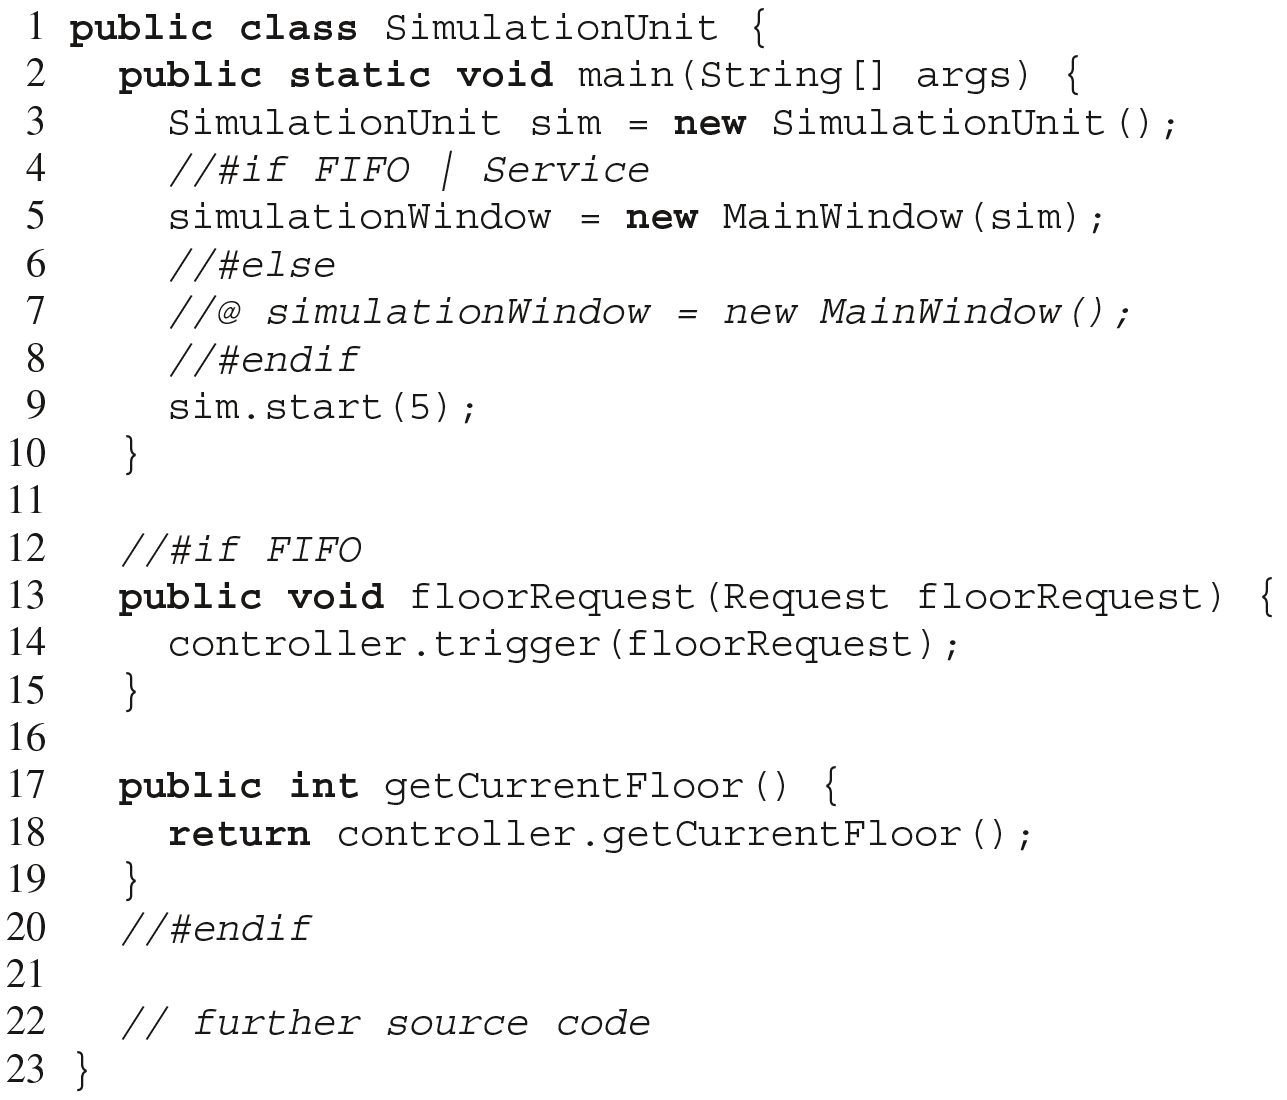
\includegraphics[width=\linewidth]{preprocessor-antenna-elevator}}
	}{
		\myexampletight{Tool Support for Feature Traceability}{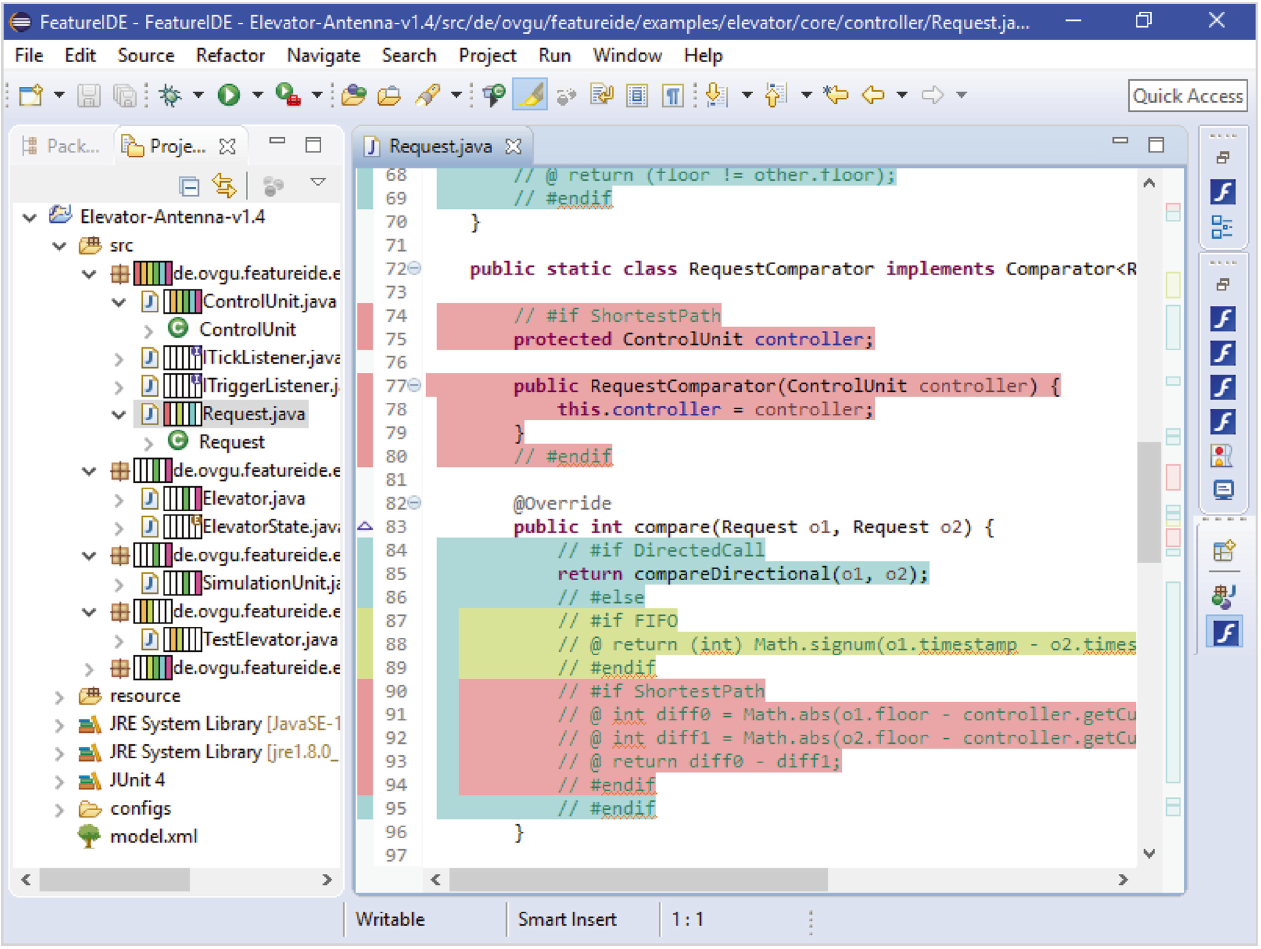
\includegraphics[width=\linewidth]{feature-traceability}}
	}
\end{frame}
% pros: fine granular, language-independent
% cons: IDE support, easy to create mistakes

\xkcdframe{619} % linux features 20s

\subsection{Preprocessor-Based Product Lines in the Wild}
\begin{frame}{\myframetitle}
	\leftorright{
		\myexample{\mysource{Liebig ICSE10}}{
			\todo{lines of code vs number of features}
		}
	}{
		\myexample{\mysource{Liebig ICSE10}}{
			\todo{number of features vs lines of variable code}
		}
	}
	\todo{add logos of all 40 systems}
\end{frame}
% TODO add pictures from Rodrigues et al. @ INFSOF’16 (Assessing fine-grained feature dependencies): methods with directives vs product lines

